% HEADER BEGINS
\documentclass[10pt, letterpaper, twoside, openany]{book}
%% Packages
\input{settings/packages}
\usepackage{graphicx}
\usepackage{float}
\usepackage{enumitem}
\usepackage{fancyhdr}
\usepackage{rotating}
%% Page Settings
\input{settings/page}
%% Own Commands
\pagestyle{fancy}
\fancyhf{}
\fancyhead[CE,CO]{\leftmark}
\fancyfoot[CE,CO]{Early Detection of MCI that progresses to dementia - An Interdisciplinary Approach}
\fancyhead[LE,RO]{\thepage}

\renewcommand{\headrulewidth}{2pt}
\renewcommand{\footrulewidth}{1pt}
\input{settings/macros}
\title{Qualifying Report}
\date{2019-01-21}
\author{Jomar Alcantara}
% HEADER ENDS
% DOCUMENT BEGINS
\begin{document}
\maketitle
\newpage
\tableofcontents
\listoftables
\listoffigures
\newpage
\chapter{Overview of Problem}
Dementia has been identified as one of those fast growing difficulties facing the world. A recent report suggests that in 2015 there were 46 million people with a diagnosis of dementia and that number is expected to hit 131.5 million by 2050 \cite{Prince2015}. The report also states that the worldwide cost of dementia in 2018 is estimated to be in the region of one trillion US dollars.
\par
In 2009, the Department of Health designed it's National Dementia strategy and as part of this made early diagnosis and support one of it's key priorities \cite{England2009}. A lot of work has gone into trying to find ways of improving the early diagnosis of Alzheimer's Disease (AD) and Mild Cogntive Impairment (MCI) with research focused on two areas - identifying biological markers and analyzing the cognitive decline of those who are suspected to have the disease\cite{Taler2008}. As described above, the numbers of those suffering from AD and MCI are going to increase as the population ages \cite{Prince2015} and thus it is important that we utilize technology wherever possible to aid clinicians in the detection of MCI and AD. At the present time diagnosis is typically conducted at memory clinics by trained clinicians\cite{Boschi2017}. I theorize that we may be able to enable an earlier diagnosis of those with MCI and AD using samples of spontaneous speech, natural language processing (NLP) and machine learning (ML).
\par
There is a large body of research that looks at the decline in language in those with MCI and AD\cite{Taler2008, Boschi2017}. However there is conflicting evidence in these studies about which declining language factors are associated of MCI and AD\cite{Taler2008, Boschi2017}. Research therefore should look at these features in more detail and a clarification of this currently disorganised picture should go some way to helping researchers further understand the disease and it's progression. One of the difficulties in research of this nature is the process of collecting appropriate language samples. Part of this work therefore is to see whether spontaneous discourse, such a semi-structured interview, has the ability to put pressure on both the cognitive and linguistic systems in the same way as traditional cognitive tests such that it might be able to distinguish between healthy controls, those with MCI and those with AD. There is some evidence to support this. Berisha et al \cite{Berisha2015}, has shown through a longitudinal language analysis of spontaneous speech that there are marked differences in this process between those who would go on to have a diagnosis of AD and a healthy control. 
\par
The potential impact of this research in this area is immense. Research has shown that early diagnosis of people with AD or MCI improves sufferers quality of life and can, in some cases, slow the progress of the disease. Early diagnosis can increase the number of research opportunities for understanding the early stages of dementia and how the disease progresses so that more research can be conducted which may, in the future, lead to new treatments and other interventions.
\par
This report is structured in the following way. A literature review of current methods of cognitive assessment of MCI, an review of how language is said to be impacted in the MCI and Early AD population and a review of NLP and ML techniques that have the potential to be applied to this domain is presented in Chapter 2. The findings from a replication and extension of previous research using an existing dataset is presented in Chapter 3. I detail the aims of my research and my proposed future work plan including distinct tasks to be completed over the next two years in Chapter 4. Finally, my conclusions are summarised in Chapter 5.  

\chapter{Literature Review}
\section{Introduction}
Alzheimer's Disease (AD) is a neurodegenerative disease in which, from a physiological perspective, the brain develops neurofibrillary tangles and neuritic plaques along with the deterioration and loss of cortical neurons and synapses. Whilst a definitive diagnosis of Dementia can only produced at post-mortem, there are a number of clinical indicators from psychological perspective that can indicate dementia is present. From a clinical psychology perspective, those who have dementia demonstrate cognitive deficits such as problems with episodic and semantic memory, organizing and planning, difficulties with language and visuospatial deficits\cite{McKhann2011}. In addition, these symptoms are often accompanied by emotional problems such as depression and behavioural difficulties. 
\par
AD and other forms of dementia affect a significant proportion of the geriatric population in the world today and is currently the sixth leading cause of death in the US and was named the leading killer of women in the UK. According to a recent report commissioned by the Alzheimer's Society in 2015, they estimate the prevalence of AD in the UK at approximately 815,000 people. This represents 1 in 14 of those aged 65 or over and 1 in 79 of the general population \cite{AlzheimersSociety2014}. From a financial perspective, they estimate an annual spend of £4.3 billion of which approximately £85 million is spent solely on diagnosis and that the total impact of AD (excluding the costs associated with early onset dementia) is £26.3 billion annually. Globally, this picture is a lot bleaker. Another report by Alzheimer's Disease International suggests that in 2015 there were 46 million people with a diagnosis of dementia globally and that number is expected to hit 131.5 million by 2050 \cite{Prince2015}. The report also states that the worldwide cost of AD in 2018 is estimated to be in the region of one trillon US dollars.
\par
Despite this growing problem, at present there are no drugs that improve the prognosis of those suffering with AD. All the drugs that are on the market are designed to manage symptoms. Whilst there are numerous investigational drugs in development for the treatment of AD, a larger than normal percentage (99.6\%) of these drugs fail in clinical trials (in contrast to anti-cancer drugs which have a 80\% failure rate) \cite{AlzheimersSociety2014}. Researchers have proposed that a possible reason for the lack of success is that the drugs treatments are initiated too far along in the progression of the disease and thus much of the degeneration of the brain has already taken place. It is therefore important to focus AD at it's earliest stages which some literature describes as 'Mild Cognitive Impairment (MCI) due to AD'.
\par
Current thinking suggests that the cognitive deficits associated with AD often begin before the clinical symptoms of the disease become apparent. Researchers propose that neurofibrillary tangles and other associated physiological effects of AD develop over time and alter cognitive function until a threshold is reached and clinical symptoms become more obvious \cite{Nestor2006}. The case of Iris Murdoch, who had a confirmed diagnosis of dementia, illustrates this theory well. Le et al \cite{Le2011}found, in their analysis of three writers and the novels they wrote, that Iris Murdoch's work declined subtly over time, but there was a steep drop off in the use of language in her last novel when, it is theorized, the symptoms of AD manifested themselves more significantly. If this theory holds true more generally, it should be possible to detect subtle cognitive changes in language and memory before a clinical diagnosis can be formed. However, one of the challenges of this approach is differentiating natural cognitive decline due to aging with decline due to a form of dementia. Albert and his team have worked to define clinical criteria which professionals can use to diagnose MCI due to AD and differentiate this from age-associated memory impairment and age-associated cognitive decline. They note that the diagnosis of MCI requires evidence of intra-individual change and optimally requires evaluation at two or more points \cite{Albert2011}.
\begin{enumerate}
	\item Concern regarding a change in cognition - A person or an informant should express concern that there is a change in cognitive ability in comparison to previous level of performance.
	\item Impairment in one or more cognitive domains - There should be evidence of lower performance in one or more cognitive domains beyond what would be expected of a person given their age and education. 
	\item Preservation of independence in functional - Whilst persons with MCI are expected to be able to maintain independence, it is common to experience mild problems in complex functional tasks which they may have been able to perform previously. This might mean that they take more time or be less efficient at completing these tasks, or it may be that may make more mistakes.
	\item Not demented - The deterioration should be mild to the point that there is no significant loss of functioning in social or occupational contexts.
\end{enumerate}
In addition to meeting the above criteria, a clinician must rule out other conditions or factors that could account for the decline in cognition with the goal to increase the likelihood that the underlying cause of this decline is AD. 
\par 
Many researchers have studied the early detection of MCI \ AD. These studies usually follow two main approaches. The analysis of biomarkers and the examination of patients who have demonstrated decreasing cognitive abilities. The first approach yields reliable results in the detection of AD in its moderate and advanced states but does not perform well during the early stages of the disease. The second approach has gained more attention in recent years, due to the fact that in clinical practice it has shown promise in the early detection of AD. In addition, the analysis of the decline of cognitive abilities is comparatively inexpensive and less invasive that the first approach which commonly requires the collection of a sample of cerebro-spinal fluid which is painful for the patient involved. 
\par
One of the most common ways in which clinicians traditionally make an early diagnosis of cognitive impairment is through the use of the Mini Mental State Examination (MMSE) \cite{Folstein1975}. The MMSE is a brief questionnaire consisting of eleven questions which tests cognitive aspects of mental function and requires only 5-10 minutes to administer \cite{Folstein1975}. The MMSE is chosen due to it's effectiveness at assessing a person's cognitive mental state at a specific point in time, as well as being as sensitive to changes as a more detailed and complex assessment such as the Wechler Adult Intelligence Scale \cite{Folstein1975}. Whilst the MMSE is useful as a brief screening tool it has it's limitations. The MMSE was not specifically created to screen for dementias and therefore does not interrogate key aspects of cognitive impairment known to be affected in dementia. It also has limited value in assessing under-educated subjects and a meta-analysis on the effectiveness of the MMSE as a diagnostic tool for dementia showed that it's accuracy was low (sensitivity between 78.4\% and 85.1\% and specificity between 81.3\% and 87.8\%). As the MMSE is shown to have low accuracy specifically in the diagnosis of dementia, it becomes necessary for professionals to employ the use of other tools or measures such as the Free Cued Selective Reminding Test (FCSRT) \cite{Grober2010} or the Montreal Cognitive Assessment (MoCA) \cite{Davis2015}. These tests have the benefits of being much more accurate at diagnosing cognitive impairment and discriminating between dementia and other types of cognitive impairment at the cost time and training of psychological professionals such as clinical psychologists in administering these tests. Given the burden on these professionals is likely to increase due to a growing elderly population or in the case of developing countries where the clinician / patient ratio is already unsustainable, it seems useful to find less burdensome ways to aid professionals in identifying those at risk of developing dementia.
\par
The two main ways in which diagnosis is performed is through assessment of memory and language. Tests of memory are classically among the most accurate ways of diagnosing dementia, however these tests suffer from the same reliance on trained clinicians to administer these tests in a clinical setting. Language however is a lot easier to collect and can be done in more naturalistic settings. As with memory, these tests can be done over time and would be able to chart a patients language degeneration over time. Given that language is less intrusive to test and requires a lot of the cognitive processes that may be impacted by AD, a lot of research has focused on measure decline in the use of language in those with AD. There are a number of difficulties to watch out for with this approach. There are a wide number of factors that are involved in language degeneration in the elderly, and consequently there will be an expected amount of variability between subjects. The administration of such tests may induce nervousness and discomfort which may impact performance, and also repeatedly administering the same language tests for differences over time may be confounded by improved performance at tasks via practice effects. However, there is enough promise in this approach such that it could help further our understanding of the disease, it's progression and the parts of the brain affected in the early stages.
\par
According to the DSM 5 \cite{AmericanPsychiatricAssociation2013}, those with mild dementia suffer from noticeable word finding difficulty. They may substitute general terms for more specific terms and may avoid the use of specific names of acquaintances. There may be grammatical errors involving subtle omission or incorrect use of articles, prepositions, auxiliary verbs, etc. Those who have progressed from Mild to Major depression also have difficulties with expressive or receptive language. They will often use general-use phrases such as "that thing" and "you know what I mean" and prefers general pronouns rather than names. With severe impairment, sufferers may not even recall names of closer friends and family. Idiosyncratic word usage, grammatical errors, and spontaneity of output and economy of utterances occur. Echolalia (meaningless repetition of another person's spoken words) and automatic speech typically precede mutism. With the wide range of deficits someone with AD can suffer, it makes sense to try to categorise these deficits in some way.
\par
One of the most famous pieces of research on the topic of language decline in dementia was by Berisha and Liss (2015) \cite{Berisha2015} who examined speeches and public interviews of former US president Ronald Reagan. They found that Reagan's speeches towards the end of his presidency suffered from difficulties in word-finding, inappropriate phrases and uncorrected sentences which are hallmarks of language deterioration associated with Alzheimer's Disease. It turned out later to be the case that he had Alzheimer's Disease. Another classical study by Snowdon et al (1996) \cite{Snowdon1996} looked at whether linguistic ability in early life was associated with cognitive function and AD in later life. They found that idea density (defined as the number of expressed propositions divided by the number of words) was a key predictor in predicting whether nuns would go on to develop AD in later life. They found that those who would go on to develop AD all had low idea density in early life and they found no AD present in those with high idea density in early life. As we can see, just with these two pieces of research the range of language deficits in those who suffer with AD are extremely variable and can differ from patient to patient as the disease progresses. The consensus among researchers that this language degeneration is typically accelerated by the presence of dementia \cite{Berisha2015} and that a potential indicator of dementia is the rate of change in which the decline occurs relative to a fixed point in time rather than a comparison across a cohort of individuals. 
\par
Emery \cite{Emery2000} completed a literature review looking at all the potential language deficits that could exist in those with AD and / or MCI. She divided these deficits into four levels of language: Phonology, Morphology, Syntax and Semantics. She proposed that language and the processes involved in language are hierarchical in nature and that language moves from simple units of construction (Phonology and Morphology), and build layers of complexity and sophistication (Syntax and Semantics). She found that people with AD generally had intact Phonology and Morphology but more impaired Syntax and Semantics. She asserted that the language forms we learn last are the first to deteriorate as we generally learn language in small simple units initially and build syntax and complexity as we are more comfortable with language.
\par
It is clear from both the clinical diagnostic criteria and supporting research that language is impacted in those with AD. However, one of the costs of analysing language is that there is a huge burden on trained practitioners, be it clinical psychologists, audio transcribers and text encoders to facilitate the process of collecting data and analysis. The field of machine learning and natural language processing has been suggested as a way to improve the accuracy and lessen the human cost of this research as well as provide new insights into the difficulties that AD suffer in terms of language decline \cite{Boschi2017}.
% -- END OF INTRODUCTION --
\subsection{Aims and Methodology}
\par
The purpose of this review is to look at the current standards of cognitive tests available that can be used as a diagnostic tool for MCI. I then go on to explore what techniques for assessing language have been used within the field of cognitive and clinical psychology. I then go on to look at what techniques have been developed in the field of machine learning (ML), deep learning (DL) and natural language processing (NLP) that might enable the automated analysis of language easier as well as an obstacles and/or limitations of current technology. Finally, I look at some studies which have already looked at the intersection of these two domains. \newline
\par
A search of the literature was conducted using ProQuest (PsychArticles), SCOPUS, Web of Science. The following results were found (Table 1). All papers were then reviewed for relevance by reading the abstract and full text where appropriate and a shortlist was compiled. An additional search through references of shortlisted papers was also conducted and any papers who upon further review appeared relevant were added to the shortlist. Papers were included where researchers used machine learning to classify participants as MCI, AD or Healthy using language. We excluded any papers that focused on other forms of dementia or cognitive impairment, as well as any papers in which the language being analysed was not English. 
\begin{table}
	\begin{center}
	\begin{tabular}{ | p{4cm} | p{1cm} | p{6cm} | p{1cm} |}
		\hline
		Database & Results & Search Terms  \\ \hline
		ProQuest(PsychArticles) & 1484 & Language AND Decline AND Dementia \\ \hline
		ProQuest(PsychArticles) & 486  & Language AND Decline AND Dementia AND Speech \\ \hline
		ProQuest(PsychArticles) & 159 & Machine Learning AND Dementia AND Language \\ \hline
		Web of Science & 1207  & Language AND Decline AND Dementia   \\ \hline
		Web of Science & 151  & Language AND Decline AND Dementia AND Speech  \\ \hline
		Web of Science & 34 & Machine Learning AND Dementia AND Language \\ \hline
		Scopus & 791 & Language AND Decline AND Dementia  \\ \hline
		Scopus & 91 & Language AND Decline AND Dementia AND Speech   \\ \hline
		Scopus & 29 & Machine Learning AND Dementia AND Langauge \\ \hline
		Scopus & 1292 & "Language Deficits" AND Dementia \\ \hline
	\end{tabular}
	\end{center}
	\caption{\label{tab:table-name}Search Terms and Number of Results.}
\end{table}
% -- END OF Aims and Methodology
\section{Existing Neuropsychological Measures of Cognitive Impairment, and Repeatable Battery of Neuropsychological Tests}
In terms of standardised cognitive tests there are two main aims. Does the test distinguish accurately between normal aging, MCI and AD (diagnostic utility) and does the test distinguish between those individuals with MCI who will then go on to develop AD and those individuals with MCI who don't then go on to develop AD (prognostic utility). This section of the literature review outlines a number of different cognitive tests that have been used to measure cognitive impairments as well as their performance in terms of both diagnostic and prognostic utility.
\par 
\subsection{Repeatable Battery for the Assessment of Neuropsychological Status}
The Repeatable Battery for the Assessment of Neuropsychological Status (RBANS) was originally developed as an assessment tool for dementia, specifically looking at detecting a characterizing very mild dementia \cite{Randolph1998}. The authors felt that there was a shortfall of appropriate measures that were sensitive enough to milder impairments as well as a number of other shortcomings of existing tests. They met a number of design goals for this new battery of tests that addressed these shortcomings. The RBANS consists of a number of sub-tests across five distinct domains.

\begin{enumerate}
	\item Immediate Memory 
	\begin{enumerate}
		\item{List Learning}
		\item{Story Memory}
	\end{enumerate}
	\item Visuospatial / Constructional
	\begin{enumerate}
		\item{Figure Copy}
		\item{Line Orientation}
	\end{enumerate}
	\item Language
	\begin{enumerate}
		\item{Picture Naming}
		\item{Semantic Fluency}
	\end{enumerate}
	\item Attention
	\begin{enumerate}
		\item{Digit Span}
		\item{Digit Coding}
	\end{enumerate}
	\item Delayed Memory
	\begin{enumerate}
		\item{List Recall}
		\item{List Recognitions}
		\item{Story Memory}
		\item{Figure Recall}
	\end{enumerate}
\end{enumerate}

However, whilst the authors claim that the RBANS is adequately sensitive in person's with MCI, other research points out that the RBANS has poor sensitivity in detecting MCI. Another drawback of this battery is the lack of executive function measures and object naming tasks. Research has shown that the RBANS has good test-retest reliability and convergent validity. However, Duff et al warned that caution should be exercised when using the RBANS in a MCI population as it has lower sensitivity in this population \cite{Duff2010}.

\subsection{Digit Span Test}
The Digit Span Test (DST) is predominantly used to measure a person's working memory capacity, specifically the capacity used to store and recall numbers. A participant is presented with a series of numbers of fixed length and is asked to recall those numbers in normal or reverse order. The series of numbers gets progressively longer until such time as a participant fails three or more times out of eight presentations.
\par
% Muangpaisan - Digit span and verbal fluency tests in patients with MCI and normal subjects in Thai community.
Research has consistently shown that MCI patients have a significantly lower digit span score in both normal and reverse order versions of this test and a study by Muangpaisan has shown that the reverse order version of this test can, to some degree, predict a diagnosis of MCI. Muangpaisan also found that Age, Gender and Education have an impact on the performance of the tests. Emrani et al found that the DST revealed no differences between specifically amnestic MCI and controls, but could differentiate between Mixed MCI and the other groups with mixed MCI recalling fewer correct responses than other groups. Notably, there was an attenuated recency effect in those with mixed MCI. \cite{Emrani2018}. Kessels identifies that that there are working memory deficits in MCI patients and these worsen with AD patients. \cite{Kessels2011} He also identified that both MCI and AD have impaired performance on all three conditions of the digit span test. No differences were found between forward and backward conditions in any of the groups. However, available tests may not detect subtle impairments \cite{Kessels2015}.
\subsection{Rey Auditory-Verbal learning test}
Rey's Auditory Verbal Learning Test (RAVLT+) looks a wide range of neuropsychological processess including short-term auditory-verbal memory, retention of information. Participants are given a list of 15 unrelated words, repeated over five different trials and are asked to repeat. Another list of 15 unrelated words are given and the client must again repeat the original list of 15 words and then again after 30 minutes \cite{}.
\par
Several studies have shown that an impairment in RAVLT score reflect well the underlying pathology caused by AD. Thus making the RAVLT an effective early marker to detect AD in persons with memory complaints. Moradi investigated to what extent the RAVLT scores are predictable based on MRI data using machine learning approaches, as well as to find out what the most important brain regions are for the estimation of RAVLT scores. They found a highly significant cross validated correlation between the estimated and observed RAVLT immediate and RAVLT Percent Forgetting. Further, they found that the conversion of MCI subjects to AD in 3-years could be predicted based on either observed or estimated RAVLT scores with an accuracy comparible to MRI-based biomarkers \cite{Moradi2017}. Another study by Schoenberg found that RAVLT to best distinguish patients suspected of Alzheimer's disease from the psychiatric comparison group.
% Schoenberg - Test performance and classification statistics for the Rey Auditory Verbal Learning Test in selected clinical samples.

\subsection{Digit Symbol Substitution Test}
The Digit Symbol Substitution Test (DSST) involves a key consisting of the numbers 1-9 and a corresponding unique symbol. Below this key is a series of numbers from 1-9 in a randomized order and repeated multiple times. The participant is asked to fill in the corresponding symbol for each number. The task requires that the participant move between the key and the randomized sequence such that  they may retrieve the correct answer from the key, hold this in short-term memory and transcribe the key in the appropriate place.
% Rosano - Digit symbol substitution test and future clinical and subclinical disorders of cognition, mobility and mood in older adults.
Among those with no disorder in cognition, mobility and mood, being in the lowest DSST quartile compared to the highest was associated with nearly twice the odds of developing one or more clinical or subclinical disorders. Associations were stronger for incident clinical disorders in cognition. Slower psychomotor speed may serve as a biomarker of risk of clinical disorders, mobility and mood. While in part attributable to vascular brain disease, other potentially modifiable contributors may be present. Further studying the causes of psychomotor slowing with ageing might provide novel insights into age-related brain disorders. Pascoe compared patients with PD with Normal Cognition (PD-N) with those with PD and MCI (PD-MCI) and healthy participants. PD-MCI pariticipants achieved significantly lower scores than other groups in the DSST task.
% Pascoe - The symbol-digit modalities test in MCI: Evidence from Parkinson's Disease Patients.
  
\subsection{Verbal Fluency}
%% In this paragraph cite Henry et al, 2004 - taken from Taler and Phillips (2008) - Henry et al, 2004 is a meta analysis
There are a number of tests that characterise this category of verbal fluency, but generally fall into two categories. Letter (Phonemic) fluency involves the generation of as many words as possible which begin with a specified letter. Category fluency involves the generation of as many words as possible that fall into a specfied category. Both these tasks impose demands on a number of different cognitive processes namely, executive function, verbal retrieval and recall, giving appropriate answers while monitoring previous answers and inhibit inappropriate responses. However, these two tasks require different strategies when attempting them. Letter fluency relies on search strategies based on lexical representations whereas category fluency requires a search for semantic extensions of a superordinate term, meaning that semantic associations within the lexicon must be intact in order for the task to be carried out successfully. \par  
There have been numerous studies which have documented the impact that AD has on verbal fluency tests in both categories. A review carried out by Henry et al, found that performance in both letter fluency and category fluency was impaired in those with AD vs controls, but found a larger effect for tests of semantic fluency.
\subsection{Naming Tests}
Word-finding difficulty is a common symptom of AD and these deficits usually occur during the early stages of the disease progression. As such , a test of a patients ability to find words (known as confrontation naming) is a common way to measure cognitive decline. One common way to do this is the Boston Naming Test (BNT) which comprises 60 items on a spectrum of very frequent to very infrequent. This has been reduced subsequently to two thirty item versions and four fifteen item versions, which correlate significantly with the original sixty item version and the benefit of the shorter versions of the test is that it facilitates testing of individuals with AD who may suffer from fatigue or limited attention span.
\par 
% Willers - Subclinical naming errors in MCI - A semantic deficit.
Willers et al studied Twenty aMCI patients, twenty AD and 21 controls matched by age, sex and education level. They found AD patients obtained significantly lower total scores on the BNT than aMCI patients and controls. aMCI patients did not obtain significant differences in total scores but showed significantly higher semantic errors compared to controls. Semantic processing is impaired during confrontation naming in aMCI.
\par 
% Vadikolias - Mild Cognitive Impairment: effect of education on the verbal and nonverbal tasks performance decline.
Vadikolias investigated the impact of education on naming tests and found that higher educational attainment in aMCI subjects were correlated with better performance in verbal and non-verbal tasks during repeated examinations over 1-year. Subjects with a lower level of education performed worse than patients with a high level of education who presented a more stable clinical score. The explanation for this is the idea of a 'cognitive reserve' in participants with a higher education such that this provides a buffer that, while not preventing the physiological symptoms of AD, can potentially delay the clinical onset of cognitive symptoms that characterise AD. This theory is supported by Snowdon who found a relationship between early life linguistic ability and the density of neurofibrillary tangles in his nun study \cite{Snowdon1996}. Whilst these studies and tests provide evidence that there are word finding difficulties in those with MCI, on their own they do not provide sufficient ability to diagnose MCI or provide an prognosis of disease progression.

\subsection{Rey-Osterrieth Complex Figure Task}
% Cite Rey 1941 - L'examen psychologique dans les cas d'encephalopathie traumatique and Osterrieth 1944 - Le test de copie d'une figure complexe.
The Rey-Osterrieth Complex Figure (ROCF) is a task widely as a test of visuo-spatial skill and visual memory. The task, which was originally designed by Rey (1944) and standardised by Osterrieth (1944) \cite{Rey1941}, asks a participant to copy a complex geometrical figure (known as the immediate copy condition and to recall and reproduce the figure from memory without warning (known as the delayed recall condition). In the immediate copy condition, the complexity of the figure requires an integrative cognitive ability. The reproduction of such a complex structure involves processes such as planning and organizational strategies that are related to executive functions.
% Salvadori - Qualitative Evaluation of the Immediate Copy of the Rey-Osterrieth Complex Figure: Comparison Between Vascular and Degenerative MCI patients.
Salvadori found that patients with vascular MCI had a worse performance in the immediate copy of the ROCF compared to individuals with degenerative MCI, despite their significant impairment in terms of general cognitive status and visual memory. Evidence shows that patients with disorders that possibly involve attention and executive functions are characterized by a more disorganised approach when copying the ROCF compared to controls. One of the difficulties with the presentation of this task in a repeated battery will be the fact that it turns from an incidental memory task (it is a memory task but the participant is not forewarned that they will be required to memorise the picture) into an intentional memory task (given the previous exposure to the task, it would be expected that a participant would pre-empt the delayed recall portion of the test and spend more time attempting to memorise the details). 
% Teng - Persistence of Neuropsychological Testing Deficits in Mild Cognitive Impairment.

\subsection{Hayling Sentence Completion Test}
Inhibitory deficits are a common in all stages of dementia. This is usually tested using Stroop test, however this has the drawback of lacking ecological validity. Therefore researchers have moved towards using the Hayling Sentence Completion Test (HCST) which uses skills such as word retreval as well as the ability to inhibit ones responses where appropriate and is therefore a much more ecologically valid task. There are two parts to the HCST. In the first part, participants have to complete a sentence by providing a word that best fits the given sentence (this is known as the initiation condition). In this second part, participants have to complete sentences by inhibiting an impulse to give the word that best first the sentence as in the first part, and producing a semantically unconnected word. Performance in both conditions is measured by the time taken for the participant to initiate a response, and in the inhibition condition also by the correctness of the word.   
\par 
% Martyr - Assessing inhibitory control in early-stage Alzheimer's and Parkinson's disease using the Hayling Sentence Completion Test.
Martyr et al compared healthy controls with patients with dementia and patients with parkinson's disease. They found that a high proportion of Category A errors (producing a word that fits the sentence when instructed otherwise) was a factor in performance loss for participants with dementia. Findings suggest that the HSCT may be sensitive to verbal suppression deficits and may provide insight into inhibitory control in participants with dementia. Patients with Dementia were significantly slower than controls in the initiation and inhibition conditions vs healthy controls, and slower than patients with parkinsons disease in the initiation but not the inhibition condition.
\subsection{Grooved Pegboard Test}
The Grooved Pegboard Test (GPT) was originally designed to cover a variety of different psycho-motor functions including hand-eye coordination and motor speed. However, some studies have shown a correlation of performance in the GPT and measures of cognitive performance such as the Montreal Cognitive Assessment.
% Bezdicek - Grooved Pegboard Predicates More of Cognitive Than Motor Involvement in PD.
Bezdicek found that the GPT predicted performance on the MoCA and concluded that in addition to being a measure of motor skills, there were results that showed that the GPT could also provide information about a participants cognitive skills. Whilst this was specifically using a population of patients with Parkinson's disease, given the MoCA and GPT have shown degree of correlation, there remains an opportunity for research that explores the use of the GPT with MCI and Early AD populations.
% Darweesh - Simple Test of Manual Dexterity can identify persons at high risk for neurodegenerative diseases in the community.
Darweesh et al, used the Purdue Pegboard Test to assess manual dexterity in a healthy older adult population and followed their participants for between eight and twelve years until an indication of the onset of a neurodegenerative disease. In this time 227 (4\%) of their participants went on to develop a diagnosis of dementia. They noted that higher PPT scores were associated with lower risk of incident neurodegnerative disease and noted significant associations of PPT scores with all forms of dementia and this potentially highlights a deterioration of motor function in the pre-clinical  phase of dementia.
\subsection{Visual Search}
The visual search task requires participants to be watching a computerised display in which a target appears either by itself or surrounded by other elements which are used as a distraction. These other elements can be vary in similarity to the target. This is inherently a measure of attention shifting and processing of various similarity and as one would expect, the visual search time is increased in the presence of distractors. This effect is magnified in participants who have a cognitive impairment. 
% Abnormal Visual Search in MCI and Alzheimer's Disease. Tales.A 2005
Research has shown there to be deficits in both AD and MCI populations in this task. Whilst these deficits were not as apparent in MCI populations, there remained a significant enough difference that could be used to differentiate healthy controls from those with MCI. In a comparison of visual search performance between those with aMCI and healthy controls, Tales noted significantly poorer performance in the aMCI group. However, she also noted a good deal of heterogeneity in the aMCI group which illustrates that whilst the aMCI group have essentially the same condition, presentations within this population can differ markedly. The results from this trial also illustrates the use of a non-memory task as a means of diagnosing dementia as patients who went on to be diagnosed with dementia whilst this study was in progress had significantly poorer visual search performance.  
\subsection{Free Cued Selective Reminding Test}
The Free Cued Selective Reminding Test (FCSRT) was borne out of the premise that by controlling the conditions of learning, a measure of memory is possible that is not confounded by normal age related changes in cognition. Theoretically speaking, any controlled learning test should be able to discriminate between cognitive decline due to age and cognitive decline due to a cognitive impairment. FCSRT-IR (The instant recall version of the Free Cued Selective Reminding Test) performance has beeen shown to distinguish patients with MCI who then went on to develop AD, from those with MCI that did not then go on to develop AD and this led the authors to define prodromal or the amnestic syndrome of the medial temporal lobe by FSCRT-IR performance (Sarazin et al, 2007. The sensitivity and specificity of the different test forms in correctly classifying patients were compared to each other using a previously established FCSRT-IR cut off score. 
\subsubsection{Conclusions}
I have looked at a number of different cognitive tests and a battery of tests that aim to have high diagnostic and prognostic capabilities in the MCI population. However, particularly with the RBANS, there lacks sufficient sensitivity in differentiating those with MCI from healthy elderly individuals such that this tool could be used with a level of confidence in a clinical setting. In regard to the tests, a common theme is a lack of studies and therefore evidence into the utility of these tests with an MCI population. However if, as researcher, we aim to investigate this population further then a benchmark battery of tests which is sensitive enough in both diagnostic and/or prognostic utility should be a goal. 
\par 
Another criticism of the current literature is the lack of consistency with regard to the experimental groups. For example, some studies focus on differentiating between an MCI group, a AD group and a healthy controls group whereas other studies may further subdivide the MCI category according to a number of factors such as Amnesic or Non-Amnesic MCI, Mixed MCI (sometimes called Multi-domain MCI in the literature). Given the inconsistency in defining the experimental groups the confusing and often conflicting results that researchers produce is to be expected. Future research should look at the standardization of the operational definition of cognitive impairment in MCI may result in more consistent predictions of progression to AD. 

\section{Types of Language Assessment}
One of the key debates when looking at how to analyse language is the type of task provided to elicit language production in participants. In the literature researchers have primarily focused on Picture Description tasks but have also suggested other ways in which we might collect data.
\par
\subsection{Picture Description Tasks}
One of the most commonly used tasks to measure language is the Picture Description task. An example of this is part of the Boston Diagnostic Aphasia Examination (BDAE), called the Boston Cookie Theft picture description task \cite{Kaplan2010}. The Cookie Theft picture (pictured below) depicts a scene of a home typical of the period of time when it was created and would generally not require participants to use any complicated vocabulary to describe. In this task participants are asked to describe the picture presented to them in as much detail as possible.  This task was originally designed to assess Aphasia, but has shown itself to be useful in the assessment of language for the purposes of diagnosis of MCI and AD as well \cite{Giles1996}
\begin{figure}[H]
\centering
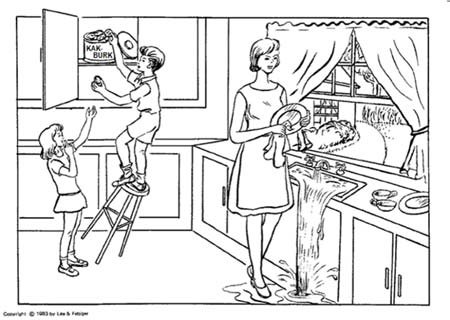
\includegraphics[width=240px, height=150px]{images/BCTPicture.png}
\caption{Cookie Theft Picture.\label{white}}
\end{figure}
\par
The picture description task does a fine job of eliciting descriptive language however because of the specific content the language produce could be considered quite limited. There is some disagreement as to the benefits of this using this methodology. This task is reported as being useful to lexico-semantic disorders \cite{Boschi2017, Sajjadi2012} as the language being generated is primarly nouns and deixis (words to identify items and words to put those items into context). However, Ash \cite{Ash2012}felt that there was no difference in using this task vs Story Narration (described below). In explaining the differences, it is worth noting that these researchers were using differing variables and this could explain their different perspectives.
\par
\subsection{Narrative description task}
The story narration task is designed to study a participant's ability to describe and elaborate on a story which is depicted using a series of pictures. The stories depicted are usually based on children's books or famous stories with the Cinderella being the one most typically used \cite{Fraser2014}. This task requires ordering the story in a structured and coherent framework. It also requires comprehension and understanding of the stories characters and the events depicted, as well as an awareness of a character's actions, motivations and internal reactions to given events. This task is particularly useful as the procedure reduces the demands on memory, due to the participant being able to access the picture book during the description and is therefore able rule out memory as a confounding variable for any results observed. As noted above, Ash \cite{Ash2012} felt that this task was interchangable with the Picture Description task. However, other research felt that this was a studier test of lexical and semantic abilities as well as syntactic complexity because this task requires interpretation and elaboration in additional to a simple description \cite{DeLira2011}. 
\par
Given the relative strengths of the Narrative description task vs Picture description task, there are few pieces of research that have used Machine Learning to analyse features from Narrative picture tasks \cite{Fraser2014}. This could be due to the availability of data and the absence of any meaningful sets of transcripts of participants performing this task. However, this could be an interesting direction to take research in the future to see if features generated from this task could be used to predict MCI or AD.  
\par
\subsection{Interviews}
Interviews can also be used to elicit language in a more natural way by asking questions to guide a conversation between speakers. There are three types of interviews: unstructured, structured and semi-structured. Structured interviews tend to produce very limited speech and therefore has never been used in this area \cite{Boschi2017}. Unstructured interviews are open ended and generally do not conform to any particular pattern. They use generic themes such as family or hobbies to guide the conversation. Whilst this is the most ecologically valid form of conversation and therefore language generation, it's unstructured nature means that the protocol cannot be consistent and therefore reproduced. Semi-structured interviews are therefore preferred over other forms of interview as a middle ground. The semi structured nature of these interviews means that there is some replicability but does not constrain the participant in answering questions.
\par
The analysis of interviews can be difficult to analyse as both the content can vary even between participants, although it can be argued that content should not affect the type of language being generated unless it is narrow topic or the participant is constrained in how they answer a given question. It is also difficult to measure as there are no pre-defined task goals in comparison to the other two methods. Nevertheless, this is the most naturalistic setting for looking at language production and can be used to look at the syntactic and semantic parts of language generation \cite{Sajjadi2012}. There have been some attempts to use interviews to assess language production in AD with promising results \cite{Asgari2017, Guinn2015}.
\par
\subsection{Conclusions}
One can view the different types of tasks above as a continuum where picture tasks represent a much more controllable task with a lot of supporting research but which generates a much more constrained set of language that is atypical of normal speech in terms of the cognitive functions used. 

\section{How do we analyse language, issues and debates}
\subsection{Single Word Language tasks vs Connected Language tasks}
Part of the reason we need to pay attention to how we ask participants to generate data is understanding how we wish to analyse the data afterwards. As discussed above, the different methodologies to collect data generate different types of language. There are two main approaches which we have looked at to analyse language, using frequencies of words and combinations of words and measures of syntax and semantics. There are other less common methods of analysing language but these are beyond the scope of this review.
\par
Single word tasks such as the Boston Naming Test and other such standardized language tests generally target a participants verbal fluency where this is defined as the ability to form and express words in accordance with certain criteria (see above for a full description of verbal fluency as task). There are a number of benefits to using single word tasks. From a research methodology perspective, using a standardized test allows researchers to target a very specific process in language generation and isolate factors that impact performance in language well. However, this approach does not take into account the symbiotic nature of language processes.
\par
Connected language tasks, such as the picture description task and interviews described above are a much more reflective of processes involved in natural language generation. They are able to be relatively constrained in the language available to be used, for example in the picture description task, or they can be unconstrained in the form of interviews. % ADD MORE!
\par
\subsection{Semantics vs Pragmatics}
When navigating the English language it is necessary to distinguish between what a sentence says in both semantic and pragmatic terms. Semantic meaning refers to the meaning of the words in a sentence local only to the given sentence. Another way to put this is, semantics considers the meaning of words without taking into account the context in which these words are spoken. Pragmatic meaning refers looks at the same sentence in terms of words and grammar but takes into account the situation or context in which these words are spoken. Emery in her literature review looks at all levels of language tasks except for pragmatics, however this is an area that should not be ignored.
\par
\subsection{Semantic Content}
Another approach to linguistic analysis in this field is the idea of measuring semantic content and complexity. According to Emery (2000) \cite{Emery2000} in which she states that Semantic and Syntactic skills deteriorate first in people with MCI and AD. If this is true, then psychological measures of semantic and syntactic skills should be able to pick up signs of deterioration and act as markers for possible MCI and AD. An example of a semantic complexity measure is the concept of idea density. Formally, idea density is defined as the average number of propositions per sentence \cite{Kintsch1973} and this was used to successfully differentiate between people who would later go on to develop AD \cite{Snowdon1996}. Some examples of semantic content measures are Type to Token Ratio, Brunet's Index and Honore's Statistic (described below) which are used to measure the lexical diversity of a given piece of text and/or utterance.  This has also shown to be effective in differentiating between MCI, AD and Controls, with those with language impairments \cite{Bucks2000} and this has carried through in research involving machine learning \cite{Wang2016, Thomas2005}.
\par
\subsubsection{Type token ratio(TTR)}
Type token ratio (TTR) is the ratio obtained by dividing the types (The total number of different words) by the tokens (the total number of words in an utterance).
\begin{equation} \label{x1}
TTR = numberOfUniqueWords / totalNumberOfWords.
\end{equation}
\subsubsection{Brunet's Index(W)} % Don't forget to cite the original article.
Brunet's Index (W) differentiates itself for TTR, as it is not impacted by the length of the text itself. Brunet's Index is defined by the following equation:
\begin{equation} \label{x2}
W = N^{V(-0.165)}
\end{equation}
where N is the total length of the utterance being measured and V is equal to the total vocabulary being used by the subject. Brunet's Index usually has a score of between 10 and 20, with high numbers indicating a more rich vocabulary compared to low numbers. \newline
\par
\subsubsection{Honore's Statistic (R)} % Don't forget to cite the original article.
Honore's Statistic is based on the idea that vocabulary richness is implied when a speaker uses a greater amount of unique words. This is indicated by the following equation:
\begin{equation} \label{x3}
%% Check to see if this is accurate.
R = (100 \log N) / (1 - V1/V)
\end{equation}
where v1 is equal to the number of unique words, V is the total vocabulary used and N is the total number of words in the utterance being measured.
\subsection{Picture-related content thematic elements}
Several studies examined the amount of thematic elements expressed that were directly relevant to picture stimulus in picture description tasks. The studies used a variety of phrases to denote these thematic elements, these included 'pictorial themes', 'relevant observations and 'semantic units' but are notionally similar. The only difference was the number of thematic elements that 'scored' for the studies in question. Nicholas et al identified eight thematic elements of the Cookie Theft picture and used the number of elements as an outcome measure in different groups. He found that patients with AD expressed significantly fewer content elements than controls.
\par
Hier, Hagenlocker and Shindler assessed content using a similar list of thematic elements. They divided their participants into early-stage and late-stage AD, as well as including a control group. The late-stage AD group produced significantly fewer relevant observations than the early stage group, and the AD group combined produced fewer relevant observations than controls. This study was replicated by Vuorinen et al (2001).
\par
Smith, Chenery and Murdoch (1989) applied Hier's methodology for constructing pictorial 'themes' with the Picnic Scene from the Western Aphasia Battery (WAB) with a control and patients with moderate to moderately severe AD. The authors found no difference in the number of semantic elements produced but did not that the group with moderate to moderately severe AD took more time and more syllables to communicate these elements.
\par
\begin{figure}[H]
\centering
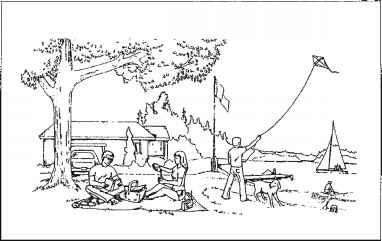
\includegraphics[width=240px, height=150px]{images/picnic-scene.jpg}
\caption{Picnic Scene taken from the Western Aphasia Battery (WAB).\label{white}}
\end{figure}
Sajjadi et al (2012) examined 10 pictorial themes in picture description the Comprehensive Aphasia Test and found that the group with mild AD produced similar themes than controls. Bschor et al. (2001) examined Cookie Theft picture descriptions at four stages of AD. They identified 12 elements of the cookie theft picture and found that whilst each AD group differed significantly from the others and from controls, the measures did not distinguish between MCI and normal controls.
\par
Finally, a number of studies used composite measures which contained thematic elements and other unspecified information units resulting in a list of 23 possible information units of the Cookie Theft picture. The authors felt that this provided a wider, more liberal range of relevant content and thus subtler differences could be noted. Studies using these features found some differences between AD and controls, and some could differentiate between different stages of AD.
\subsection{General Information Units}
Some studies used a more general concept of content, defining "information units" as "the smallest non redundant meaningful fact or inference," whether or not the information conveyed was specific to the context in which the conversation happened. Giles et al, for example, studied adults with minimal, mild or moderate AD vs controls and found that adults with AD produced fewer overall information units than controls.
\subsection{Conciseness of information}
Conciseness has been defined as the number of words a speaker uses to express ideas. The theory is that people with AD will need more words to convey ideas because of word-finding related behaviours such as circumlocutions and repetitions. Conciseness is calculated by dividing the number of ideas expressed by the total number of words in a measure commonly referred to as idea density but also known as lexical index, information content and information unit conciseness index. Snowdon et al examined written discourse from the Nun study and found that low idea density in early life was associated with reduced cognitive performance in later life. Riley et al extended these findings by concluding that early-life idea density was associated with lower brain weight, higher degree of cerebral atrophy and increased neurofibrillary pathology in later life.
\par
Ahmed, de Jager et al examined idea density with patients who had confirmed AD post mortem. They found that those with AD produced fewer total semantic units than controls but there was no significant difference between the groups with regards to idea density. The study of "empty speech" by Nicholas et al examined conciseness with measures thought to contribute to the "nonspecifity" of discourse in AD, such as empty phrases (defined as common idioms contributing no relevant information), deictic terms (e.g. "this", "that" without referents), indefinite terms (e.g. "thing" or "stuff"), pronouns without proper noun antecedants, and repetitions. In their study they found that AD patients produced more of these behaviours than did controls.
\par
\subsection{Efficiency}
Efficiency is the rate at which meaningful information is conveyed over time, calculated by dividing the total number of information units by the duration in seconds of the speech sample. Smith et al, 1989 found that 18 adults with moderately severe AD produced fewer content units per minute on average than controls, and attributed this different to increased circumlocutions and repetitions. Murray 2010, used an analogous measure which he called "performance deviations per minute", in which fillers, irrelevant words, revisions or false stars, vague or non-specific vocabulary and inaccurate output (e.g. paraphasias) were divided by the total number of minutes in the speech sample; this measure was lower for those with AD than those with depression, and also healthy controls. The authors suggested that discourse information measures may help disentangle the similarities in symptoms of early AD versus depression in older adults. Guinn (2012, 2015) \cite{Guinn2012, Guinn2015} found that 'Go-ahead utterances' - instances in dialogue in which a speaker provides responsees do not add anything in a conversation beyond a minimal response, were significantly more frequent in those with AD than healthy controls.
\subsection{Quantity - Total number of words}
Several studies report that adults with moderate AD produce fewer words than controls on picture description, however other studies found no differences in total words among groups of controls and patients with MCI or AD. Murray and Nicholas et al investigated normal controls, patients with AD and older adults with depression and found no group differences in total words. In contrast, Lira 2014 found that controls produced more total words than patients with AD but found no difference between mild and moderate groups.
\par
\section{Syntax and Morphology (Language Form)}
Syntax can be defined as the rules that govern how words can be combined to form sentences, whilst Morphology is the system that governs the structure of words and the construction of word forms. Multiple studies of language decline in dementia included at least one measure of syntax or syntactic complexity. Common constructs included words per clause, grammatical form (measures of an appropriate use of syntactic conjections, tenses, conditionals, subordinate clauses and passive constructions), measures of phrase length and proportions of words in sentences. Some researchers have explored the use of formulaic language in those with dementia, the theory being that well practiced phrases are less effortful and therefore place low load on the cognitive abilities of those with AD. The general hypothesis motivating these studies is that either working memory limitations or semantic memory limitations in AD affect one's ability to use complex constructions.
\par
\subsubsection{N-grams}
One of the first features discussed as a potential predictor of MCI or AD is the n-gram. An n-gram is a contiguous sequence of n items from a given sample of text or speech. The items can be phonemes, syllables, letters, words or base pairs according to the application. For example, given the sequence of words "to be or not to be", this extract is said to contain six 1-gram sequences (to, be, or, not, to, be), five 2-gram sequences (to be, be or, or not, not to, to be), four 3-gram sequences(to be or, be or not, or not to, not to be) and so on. This is useful as, given a large portion of text or speech, we can predict the probability of a word being close by to a given word. A number of researchers have used n-grams as features. 
\par
Asgari, Kaye and Dodge (2017) \cite{Asgari2017} used another form of word frequency measurement. Using recordings of unstructured conversations (with standardized preselected topics across subjects) between interviewers and interviewees they grouped spoken words using Linguistic Inquiry and Word Count (LIWC) which is a technique used to categorize words into features such as negative and positive words \cite{Pennebaker2015}. They were able to successfully used machine learning algorithms to distinguish between these two groups with an accuracy of 84\%. 
\par
\subsection{Mean length of utterance (MLU)}
Murray found that MLU was not a distinguishing factor among health adults, adults with depression and adults with AD. Ripich et al found a decrease in MLU in adults with severe AD over time, and this was supported by findings of Le et al in their studies of authors \cite{Le2012}
\par
\subsection{Proportion of verbs to nouns plus verbs}
Kave and Levy used a verb index to capture syntactic complexity and found that adults with AD expressed the same amount of verbs to nouns plus verbs as adult controls.
\par
\subsection{Syntactic Complexity - Composite measures of MLU, syntactic errors and verbs}
Ahmed et al, and Ahmed, Haigh et al found differences in syntactic complexity between adults with MCI and controls, and between MCI and moderate AD stages. The differences in syntactic complexity were not significant when individual measures were tested, but were apparent using a composite score consisting of MLU, words in sentences, syntactic errors, nouns with determiners, and verbs with inflections.
\par
\subsection{Formulaic Language}
Fraser, Meltzer and Rudzicz (2015) \cite{Fraser2015} looked at connected speech using the DementiaBank corpus. They found that there were four factors which informed the classification of participants as either healthy or AD. These four factors were semantic impairment, acoustic abnormality, syntactic impairment and information impairment and were based on existing measures of semantic and syntactic complexity. Zimmerer (2016) \cite{Zimmerer2016} looked at whether language was more formulaic in those suffering from AD. He proposed that those who suffer from AD rely on formulatic sentences, for example 'Noun-Verb-Noun', and this is done to reduce language complexity. He noticed a significant difference in the use of formulaic sentences between AD and Healthy Controls.
\par
\section{Pragmatic Language}
The pragmatic language domain refers to the social rules for language for the purposes of communication including, using language to achieve goals, using information from the context to achieve these goals and using the interaction between people to initiate, maintain and terminate conversations.
\subsection{Questions, turn-taking, unsure statements, egocentric comments}
One study, Ripich et al, examined several pragmatic abilities among patients at different stages of AD. The severe AD group asked more questions over time than the other group. The authors argued that question-asking was a compensatory strategy, and as a result, adults in late-stage AD may have had insight into their communication problems. Potentially, there were a number of flaws of the methodology if their research. Firstly, a caregiver was asked to administer the picture description task in order to mirror a more typical communicative interaction. Whilst this improved the ecological validity of the study, the caregivers delivery would be varied and inconsistent. Secondly, due to the constrained nature of the picture description task, it is unlikely that it would be able to capture the pragmatic skills that are typioical of conversations in everyday life.
\par
\subsection{Coherence}
Coherence refers to the appropriate maintenance of topic in discourse and is thematically related to the immediately preceding utterance (local coherence) and by how closely an utterance relates to the general topic at hand (global coherence). One study looked at coherence, Chapman et al used picture descriptions of Norman Rockwell prints within a frame analysis, with frames being defined as internalized knowledge structures. The authors identified aspects of content, including typical frames of interpretation, atypical, incorrect or no frames, propositions supporting frames and propositions disrupting frames as measures of coherence. They examined these variables with early stage AD, old-elderly and normal controls. Old-elderly and normal controls produced significantly more typical frames and more frame supporting information that the AD group. The authors attributed AD patients' difficulties to memory deficits, attentional deficits, visual perceptual problems, disruption of internalized frame representation, or failure to access frame knowledge.
\par
\subsection{Perseveration}
Perseveration can be broadly defined as the repetition of a response regardless of the absence or cessation of stimulus which could have generated an appropriate response in the first place. A typical example could be the idea of conversation moving from introductions to a more general conversation, someone who has difficulties with perseveration will struggle with the move between social contexts and repeat language that would be more used in an introduction context.
\par 
One study examined verbal preservation in the description of Norman Rockwell prints, dividing the total number of words within perseverations by total number of words in the speech sample. The authors also calculated rate of perseveration on two other language tasks: confrontation naming and generative naming. Across all tasks, the AD group produced significantly more perseverations than controls; however, on the picture description task alone, there were no significant differences between the two groups. The authors theorised that this was because picture description was an easier task because there was the visual stimulus, similar to the argument made by Bschor et al \cite{Bschor2001}.
\par
\subsection{Speech intonation / prosody}
There are a number of studies, that have examined "melodic line", which is a subjective measure of speech prosody defined as "the appropriate use of intonational contour, including alterations in pitch, volume and duration". For instance, Forbes-McKay compared melodic line using a "simple" picuture such as the Cookie Theft picture vs a complex picture. The number of pictorial themes differentiated the simple tasks from the complex. Results showed no group differences on simple picture tasks (Cookie Theft and Tripping Woman) but there were differences in melodic line for the complex picture tasks. Fraser et al examined several acoustic features of speech in patients with AD ussing machine learning methods that captured both rate and phonation patterns, and found acoustic abnormalities to be a significant factor. Konig et al, also used an automated feature analysis examining vocal and temporal aspects of speech among controls, and patients with MCI or AD, and reported a classification of 81\%.
\subsection{Discourse Fluency}
Verbal fluency is a term used in neuropsychological contexts generally referring to timed, word-generation tasks, while in speech-language pathology contexts, "fluency disorders" are defined as interruptions int he flow of speaking characterized by atypical rate, rhythm and repetitions in sounds, syllables, words and phrases. "Fluency", in the literature of discourse of adults with AD, typically refers to the smoothness or flow of spoken language. Abnormalities of fluency in this population are typically characterised by filled and unfilled pauses, word repetitions, circumlocutions, and revisions. In contrast with fluency disorders (i.e. stuttering), abnormalities in the fluency of adults with MCI or AD are rarely manifested at the phonological level.
\par
The study of "empty speech" by Nicholas et al was one of the first to examine aspects of fluency in the connected speech of persons with AD. They found that adults with AD had significantly more repetitions than controls. Similarly, Tomoeda et al found more aborted phrases, revisions and ideational repetitions in the AD group than in controls. Several other studies support the idea that in AD population there are a greater number of repetitions and revisions than in healthy controls. However, there are some studies which contradict these findings (Ahmed et al).
\par
\subsection{Speech Monitoring}
Speech monitoring is related not only to word retrieval deficits and to pragmatic language skill but also to "anosognosia" define as the awareness of one's own deficits. McNamara et al investigated word error monitoring skills by comparing uncorrected and repaid errors in adults with AD vs health controls. The AD group was equally impaired in error monitoring as the controls. Severity of naming deficits correlated negatively to the amount of uncorrected errors. The authors suggested that this impairment was related to the executive function dificulties in the clinical groups. The authors did not report correlations between error monitoring and executive function test scores, however, which could have strengthened that hypothesis.
\par
Another measure of speech monitoring used in the picture description literature is "response to word-finding delays," defined as "whether patients appear unaware of their problem, produce an approximation of the target word or actively search and produce the target word". Response to word-finding delays differed significantly between minimal  AD and normal controls (forbes-McKay and Venneri). The measure was based on Goodglass and Kaplan's scale for rating discourse on the Boston Diagnostic Aphasia Examination (BDAE) and is composed of clinical judgement of behaviour that is rated on a likert-type scale ranging fdrom 1 to 7 (7 being no abnormality).
\par
\subsection{Conclusions}
This section has looked at a number of different attributes which researchers have cited as being important in the detection of MCI and AD. Whilst in some cases there is a broad consensus about a given feature in the vast majority of cases there is some uncertainty. Some of the difficulty lies in different approaches used particularly around the criteria for experimental groups which means that it is difficult to be able to compare studies, like for like, as the populations of the participants being studied vary in subtle or obvious ways. It is important for any studies moving forward to use comparable standards when it comes to their experimental groups, such that the picture can be made clearer.

\section{State of literature into Machine Learning and Natural Language processing techniques}
As we can see, diagnosing dementia through analysis has a large background in terms of psychological research. However, increasingly current research has called for the use of machine learning as a way of assisting in the process of diagnosis \cite{Boschi2017}. This section will look at what areas of machine learning could potentially be used as tools to help in this domain as well as any research that has applied machine learning to this problem.
\subsection{Natural Language Processing}
Natural Language Processing as a topic can be defined as the intersection between Machine Learning and Linguistics and looks at 


Generally speaking, Natural Language Processing (NLP) systems mimic the semiotic perspective on language. That is to say that we can subdivide NLP processes into different components (see Figure 2.3) and model broadly fits with the literature review conducted by Emery \cite{Emery2000}.
\begin{enumerate}
	\item Morphological/Lexical: providing the basic language elements or vocabulary, such as words, their roots and inflections.
	\item Syntactic: for grouping and sequencing elements within samples of language (usually sentences).
	\item Semantic: for knowing the meaning of an utterance, usually defined in terms of the 'truth value' of the logical propositions that are thought to be expressed by sentences.
	\item Pragmatic: for understanding the context and purpose of an utterance.
\end{enumerate}
\begin{figure}[H]
\centering
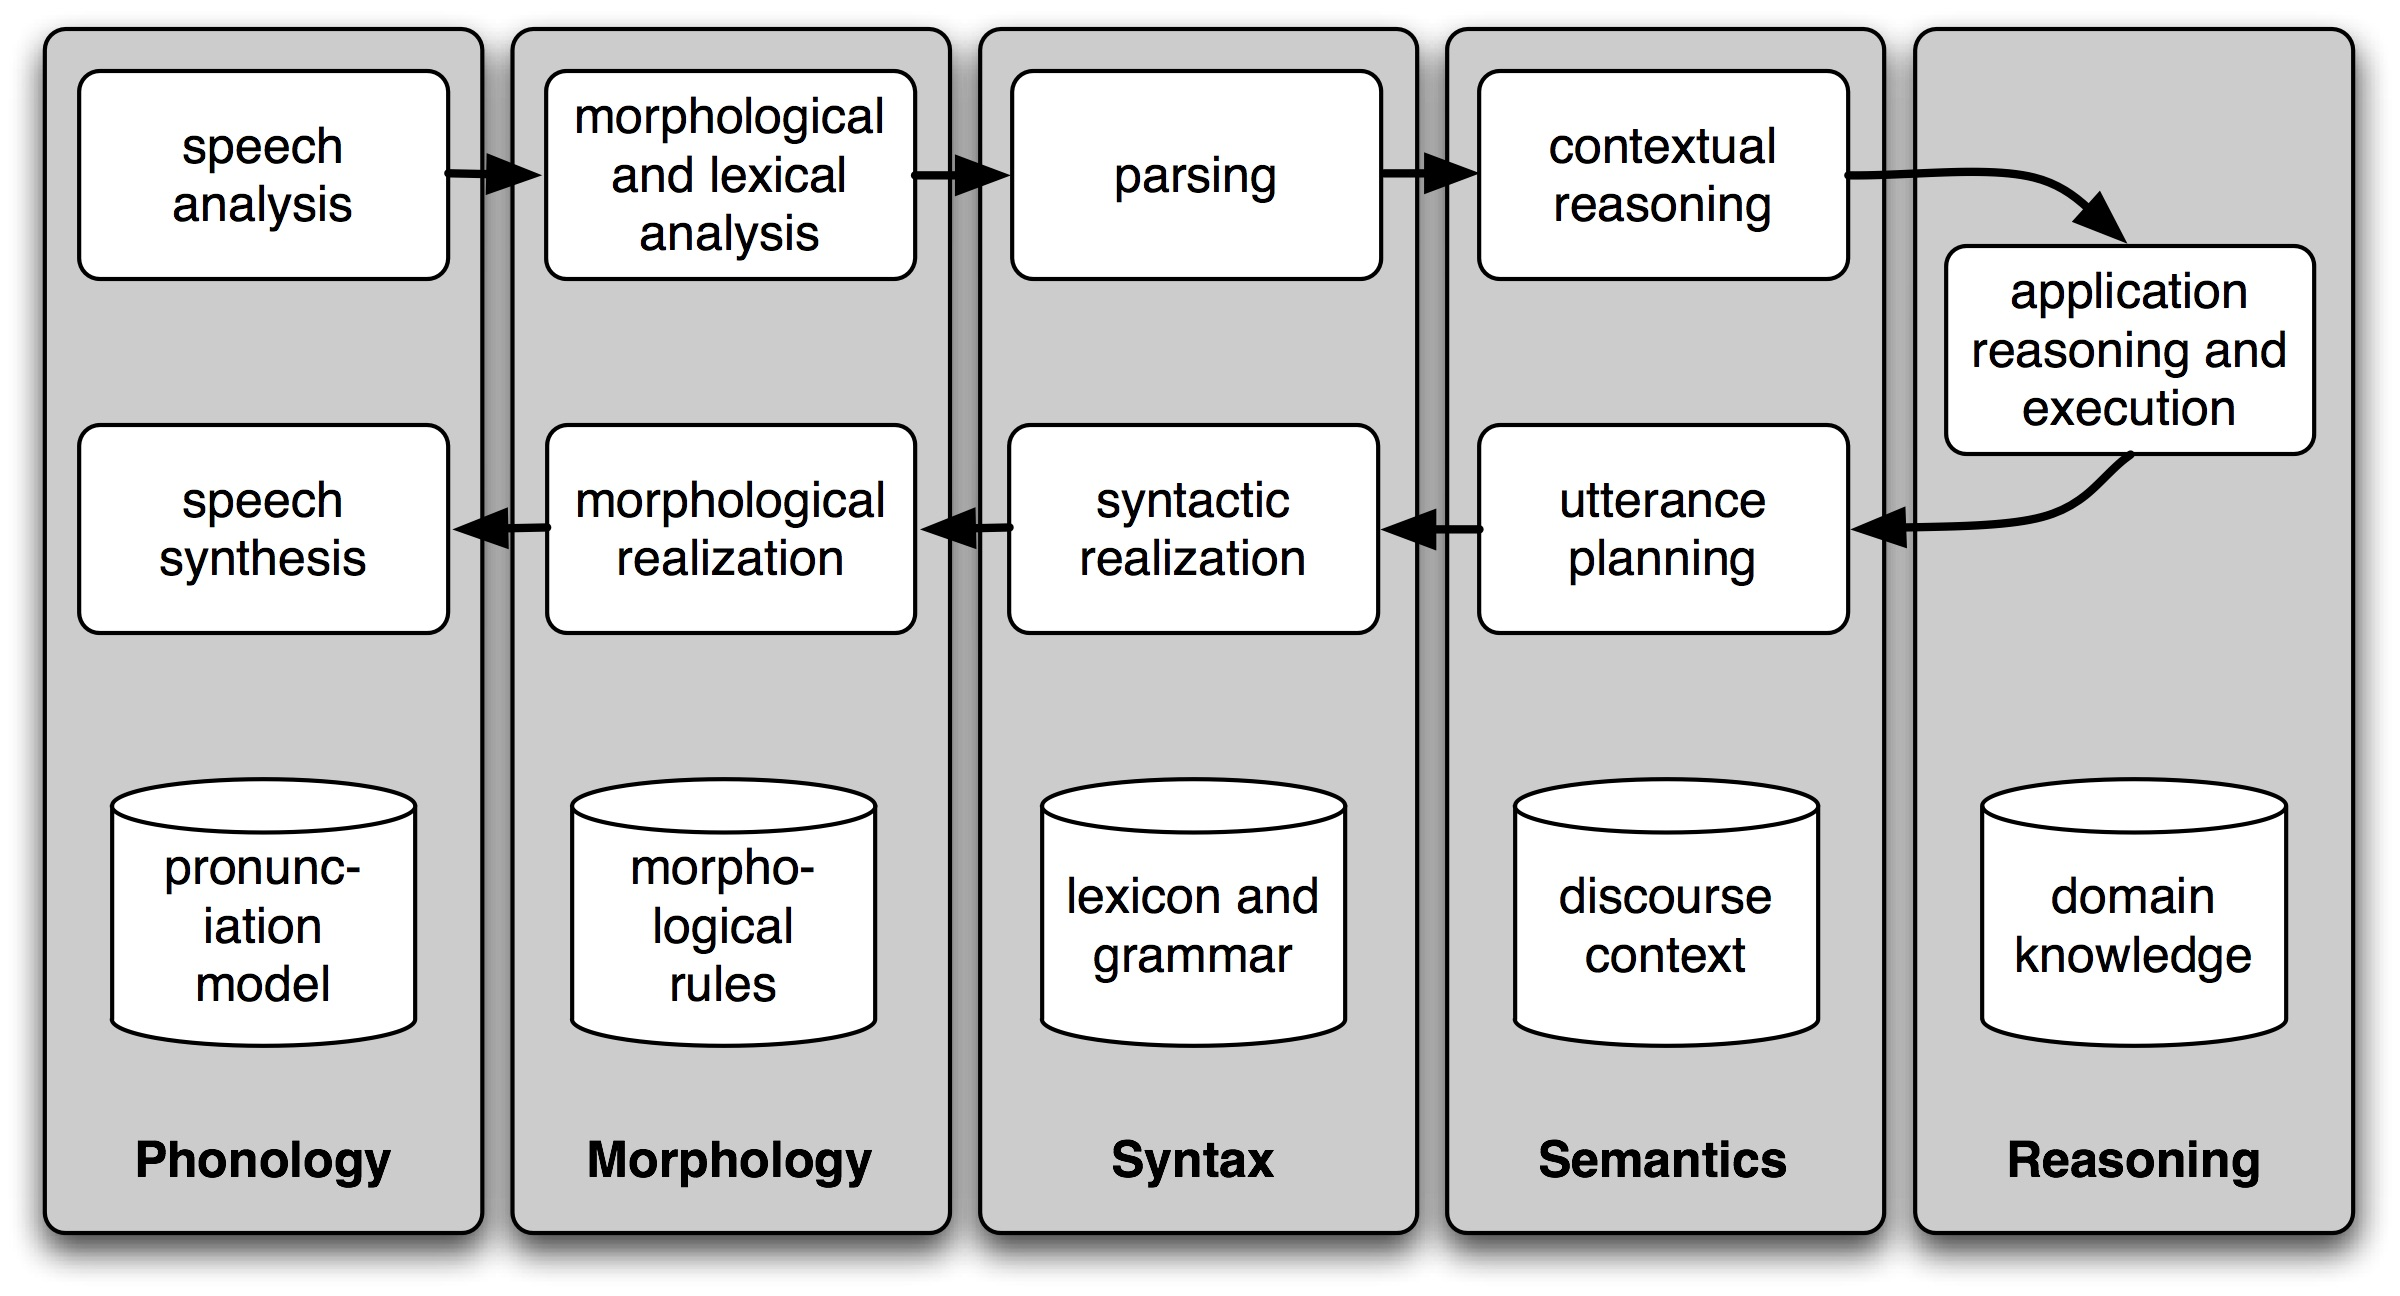
\includegraphics[width=240px, height=150px]{images/workflow.jpg}
\caption{How Natural Language Processing tasks are subdivided.\label{white}}
\end{figure}

\subsubsection{Natural Language Toolkit}
% CITE Bird, Steven, Edward Loper and Ewan Klein (2009). Natural Language Processing with Python.  O'Reilly Media Inc.
The Natural Language Toolkit (NLTK) was originally designed as part of a computational linguistics course but has evolved to become an open-source framework which includes methods and modules for a wide array of Natural Language tasks (see Table 2.2 for a full list).

\begin{table}
	\begin{tabular}{ | p{4cm} | p{7cm} | p{1cm} |}
		\hline
		\textbf{Language processing task} & \textbf{Functionality} \\ \hline
		Accessing corpora & standardized interfaces to corpora and lexicons \\ \hline
		String processing & tokenizers, sentence tokenizers, stemmers \\ \hline
		Collocation discovery & t-test, chi-squared, point-wise mutual information \\ \hline
		Part-of-Speech tagging & n-gram, backoff, Brill, HMM, TnT \\ \hline
		Machine Learning & decision tree, maximum entropy, naive Bayes, EM, k-means \\ \hline
		Chunking & regular expression, n-gram, named-entity \\ \hline
		Parsing & chart, feature-based, unification, probabilistic, dependency \\ \hline
		Semantic interpretation & lambda calculus, first-order logic, model checking \\ \hline
		Evaluation metrics & precision, recall, agreement coefficients \\ \hline
		Probability and estimation & frequency distributions, smoothed probability distributions \\ \hline
		Applications & Graphical concordance, parsers, WordNet browser, chatbots \\ \hline
		Linguistic Framework & manipulate data in SIL Toolbox format \\ \hline
	\end{tabular}
		\caption{\label{tab:table-name}NLTK tasks and functionality}
\end{table}

\subsubsection{CoreNLP}
The stanford parser is

Stanford CoreNLP provides a set of human language technology tools. It can give the base forms of words, their parts of speech, whether they are names of companies, people, etc., normalize dates, times, and numeric quantities, mark up the structure of sentences in terms of phrases and syntactic dependencies, indicate which noun phrases refer to the same entities, indicate sentiment, extract particular or open-class relations between entity mentions, get the quotes people said, etc.

Stanford CoreNLP’s goal is to make it very easy to apply a bunch of linguistic analysis tools to a piece of text. A tool pipeline can be run on a piece of plain text with just two lines of code. CoreNLP is designed to be highly flexible and extensible. With a single option you can change which tools should be enabled and disabled. Stanford CoreNLP integrates many of Stanford’s NLP tools, including the part-of-speech (POS) tagger, the named entity recognizer (NER), the parser, the coreference resolution system, sentiment analysis, bootstrapped pattern learning, and the open information extraction tools. Moreover, an annotator pipeline can include additional custom or third-party annotators. CoreNLP’s analyses provide the foundational building blocks for higher-level and domain-specific text understanding applications.


\subsubsection{Linguistic Inquiry and Word Count}
The premise behind the Linguistic Inquiry and Word Count (LIWC) is the words we speak inform an observer of the state of mind of an individual. To this end, the creators have constructed a framework which uses a dictionary of words which are pre-categorised. 
% Al-Mosaiwi - In an Absolute State: Elevated Use of Absolutist Words Is a Marker Specific to Anxiety, Depression, and Suicidal Ideation 
A typical example of this might be someone with depression who may typically be more inwardly focused and therefore talking in the first person is common. 
% Sonnenschein - Linguistic analysis of patients with mood and anxiety disorders during cognitive behavioral therapy
The 2015 version of the LIWC has over 90 different categories and some supporting research suggests that it is effective at identifying themes and associating these themes with mental health difficulties such as depression and anxiety. 
\par
A framework like this could be used as another tool to explore themes within a persons speech.


\subsection{Traditional methods of Machine Learning}

In terms of Machine Learning research in this area, a number of researchers have used transcripts based on picture description tasks \cite{Zimmerer2016, Orimaye2017, Mueller2018a, Fraser2015} and have successfully extracted linguistic features that could differentiate between AD and controls.
\par
% Thomas - Automatic Detection and Rating of AD through the Lexical Analysis of Spontaneous Speech
Thomas et al, detail several lexical approaches to the problem of detecting and rating DAT. The approaches rely on character n-gram techniques but also explore correlation of usage of frequency of different types of speech. Their results act as a proof in concept of the utility of using a pure computational approach to the diagnosis of dementia using spontaneous speech. Results - 95\% accuracy dementia vs controls. 70\% accuracy classifying dementia into two categories. 50\% accuracy classifying dementia into four categories. They suggest further exploration of characteristics to classify.
% Bucks et al - Analysis of spontaneous, conversational speech in dementia of the Alzheimer's Type: Evaluation of an objective technique for analyzing lexical performance.
AD patients had higher mean P rate, A rate and V rate scores but lower N rate scores vs normal older controls \cite{Bucks2000}.
One of the first attempts to use machine learning and natural language techniques to look was conducted by Thomas \cite{Thomas2005} who was able to successfully demonstrate the ability of machine learning algorithms to analyse n-grams as well as other features to outperform a naive rule-based classifier which always selects the modal class. Orimaye et al (2017) \cite{Orimaye2017} investigated the use of machine learning algorithms to detect differences primarily in n-gram use to distinguish between those with a diagnosis of AD and healthy controls. Their main finding supported n-grams as the most significant predictor. One of the criticisms is the use of picture description tasks and n-grams. Because the language generated by this task is content specific the n-grams generated are only specific to the task given and cannot be generalised.
\subsection{The case for Deep Learning}
% Deep Learning is an NOT 

% One of the main benefits of deep learning is that it does not rely on pre defined features being fed to the model, instead generating it's own features. This move away from relying on features solves one of the difficulties with  


% One of the drawbacks of attempting to use natural language processing and machine learning in this context is the lack of data.

\subsection{Conclusions}
We can see that both Natural Language Processing and Machine Learning techniques have a lot to offer, Indeed there has been a lot of research which have used pre-existing datasets to explore this area with promising results. To date, there has not been much in the way of research in which these techniques are applied to newly created samples of language. 

\section{Discussion}
Current state-of-the-art diagnostic measures of AD are invasive (CSF analysis), expensive (neuroimaging), and time-consuming (neuropsychological assessment). Furthermore, these measures are limited to speciality clinics and thus have limited accessibility as frontline screening and diagnostic tools for AD. More importantly, nonspecialists are often inaccurate at identifying early AD and MCI. Thus, there is an increasing need for additional noninvasive and/or cost-effective tools, allowing effective frontline identification of subjects in the preclinical or early clinical stages of AD who could be suitable for monitoring in speciality clinics and for early treatment. Implementation of effective screening instruments will allow diagnosis earlier in the course of dementia, even at the point when memory function is still essentially within the normal range. This strategy would enable an earlier, and potentially more effective, prevention and treatment of AD with a special focus to preserve cognitive functions.
\par 
However the literature has identified a number of challenges when approaching this problem. Firstly, the clinical features that combine to meet the diagnostic criteria for Dementia or it's variants are continuous in nature and heterogenous between patients and are also impacted by other variables. For example as shown above cognitive performance is affected in part by a patients educational attainment and a patients ability to live independently is impacted by a their physical health as much as their cognitive health. The challenge therefore is to find features that are minimally impacted by other factors, or that can be controlled for by a experimental design such as a matched pairs design to control for educational attainment.
\par 
Another challenge lies with the recruitment of suitable individuals who may notice a decline in cognition to the point where we might classify them as having MCI, but these individuals deduce that there is little to no value to admitting there is a problem and seeking help whilst their symptoms are 'manageable'.
\par
Finally there is a large amount of variability in the presentations of those with MCI and early dementia, and this is compounded by an similar amount of variability in the criteria researchers have used for experimental groups and the approaches researchers have used to tackle this problem. This had led to a confused literature. Recently a call for research that has consistent inclusion / exclusion criteria has been made along with some proposed definitions of MCI and it's subgroups \cite{Petersen2014}. Researchers have identified the analysis of language impairment as an area of promise to explore in the diagnosis of MCI and early AD and recent developments in natural language processing and machine learning techniques have the potential to assist in this research. Indeed, given the increased burden on the diagnosis of MCI and AD on professionals there has been a call to use technology to potentially ease this burden \cite{Boschi2017}. A small but growing amount of research has gone into the use of machine learning techniques to potentially look at the automated classification of participants with MCI and/or AD, however this is a new area of research and there are some gaps in our knowledge.

\subsection{Future Work}
One of the areas for research to study is a careful examination of the features that are being used to measure language deterioration. For example, Zimmerer (2016) \cite{Zimmerer2016} describes connectivity in such as a way that correlates directly with what Mueller (2018) \cite{Mueller2018a} calls Fluency. Whilst these are very nuanced measures which differ slightly in the form they take, the sheer range of measures and features being produced make it difficult to conceptualise as part of the larger problem. Some work needs to be done in producing a consistent list of measures that are validated using existing datasets and can be used for future research moving forward. \newline
\par
Teng et al suggests that work should focus on the MCI population and concentrate on developing a consensus neuropsychological battery that could yield predictable rates of progression to AD. This, in conjunction with the development of a model of language, sensitive enough to detect subtle deterioration in language use to act as an additional cognitive marker to aid diagnosis could potentially move some way to providing this.
\par 
Future research should also be directed towards developing non-intrusive ways of detecting subtle changes in natural language such that any perceived deterioration that could indicate the presence of MCI or AD could be flagged up early. Machine learning approaches seem to be the most logical approach for achieving this aim as language could be collected in non-intrusive ways and passed to a machine learning algorithm for preliminary classification.  Further, despite the excellent quality of datasets being used to 'backtest' these algorithms, further research should look at generating additional datasets to increase the validity of the results found so far as well as using other methods to generate data other than Picture Description tasks which we could claim are limited in scope. Finally, the recent resurgence in the use of neural networks and deep learning could provide the answer to the confused literature in terms of features. A key benefit of deep learning is it's ability to automate the process of feature engineering. So there is an opportunity to explore the use of deep learning, to not only develop new features but also  
\par
This area of research is extremely promising in its early results and the impact of successful research would be life changing for both individuals and the health of the worlds aging population in general.

\chapter{Initial Study of the Presidents corpus}
\section{Background}
There has been a significant research in the area of language deterioration as a means of detecting Alzheimer's Disease. This usually takes the form analysis of speech recorded as part of a cognitive assessment such as the Picture Description Task \cite{Orimaye2008}. Given that language samples are the relatively easy to collect, research has moved towards analysis of spontaneous speech. An good example of this type of research is the study conducted by Berisha and Liss which looked at the differences in language use between two US presidents, Ronald Reagan (who would go on to receive a diagnosis of Dementia) and George H.W. Bush who acted as a matched control based on Age \cite{Berisha2015}. They found several differences in language use which they felt acted as indicators of Reagan's difficulties with language due to dementia. These significant differences were in the number of unique words used per speech, the use of non-specific nouns and fillers and low-imageability verbs \cite{Berisha2015}. 
/par   
This study replicates work done by Berisha and Liss and extends this by adding Donald Trump as an alternative, more appropriate comparison to Ronald Reagan as he is much closer in age than George H.W. Bush. This experiment will look at the features originally identified by Berisha and Liss, as well as any others that have potential as discussed in the literature review above. 
\section{Methods}
I took 46 transcripts of Ronald Reagan’s (RR) press conferences from 1981 to 1988 and compared them with 134 press conferences by George H. W. Bush (GHWB) and 25 press conferences conducted by Donald J. Trump (DJT).  I analyzed transcripts for lexical features shown to change longitudinally with dementia  (for a comprehensive review of these, see the literature review above). For this collection of documents, I generated a number of features which looked at a number of different aspects of each document. These features encompassed, word level, sentence level and document level features and included a number of features contained in the study by Berisha and Liss with the aim of replicating and extending on their findings. These findings were. number of unique words, non-specific nouns and fillers and low imageability (LI) verbs. Imageability is characterized, according to Berisha and Liss, as the ease with which a term gives rise to a sensory .mental image. I compared the trends described in the transcripts of RR and GHWB, but also included DT. Berisha and Liss originally made the comparison as it GHWB (GHWB - age at the start of presidency - 64 years, 222 days) was the closest match to RR in terms of age (RR  - age at the start of presidency, 69 yeaars and 349 days). However, with the inauguration of Trump, he now is the closest comparible president in terms of age (DJT - age at the start of presidency - 70 years, 220 days). It would be interesting to look at a comparison of RR and DJT to see whether the comparisons made by Berisha and Liss hold true with this more appropriate match (in terms of age). DJT as with GHWB has no known diagnosis of AD. I used the press conference transcripts in the American Presidency Project (APP) archive as a data source for this project. The APP is a comprehensive and organized searchable database of presidential documents, including transcripts of speeches, transcripts of news conferences, and other public documents.
\subsection{Pre-processing}
To generate the files necessary for analysis, I downloaded each transcript and performed the following changes. I omitted the prepared statement by the president and any speech by other individuals. I started each transcript at the beginning of the first answer to a question. I filtered any annotations that were added to the transcript, including any references or clarifications, and any laughter. It's worth noting that there appears to be a difference in how 'hesitations' were marked down between each president, for RR hesitations were marked by a single hyphen whereas for GWB hesitations are marked by a double hyphen. In order to maintain consistency when parsing through the documents, I have changed both types of hesitation to be marked by a single hyphen. I also omitted one word sentences as this data would, from a theoretical perspective, not be relevant for language analysis. I did not control for the length of the document, but generated features which would normalise by the length of the document. I therefore was able to include all press conferences by both Ronald Reagan and George H.W. Bush where there was a question and answer session conducted at least in part by the sitting president (2 press conferences of GWB were ommited due to a lack of a question and answer session).
\subsection{Feature Selection}
\section{Results}
\section{Discussion}
\section{Conclusion}



\chapter{Future Work}
\section{Introduction}
This section looks at my research aims and objectives given the literature review presented above. This section will then go on to explore any challenges to my research. I then present the work I have planned for the next two years, divided into distinct tasks with their own aims and objectives. As part of this I will identify target conferences where I could present my work. Finally, I look at potential risks and ethical concerns that could conceivably occur.
\section{Research Aims and Objectives}
The aim of my research is to ultimately to identify less burdensome ways of detecting dementia without the use of invasive procedures (taking bloods, or using medical equipment such as MRI's and EEG's) and without resorting to time-consuming and expensive psychological tests. There is a lot of research into the analysis of language as a marker for MCI \cite{Taler2008, Boschi2017} and there have been calls for research that explores the use of Natural Language Processing and Machine Learning techniques to aid in the analysis of language \cite{Boschi2017}. This will be the focus of my research.
\par
I have deliberately selected the MCI population as examining language decline at this stage has the potential to further our understanding of how MCI progresses into dementia. Given that sampling a person's language is relatively effortless, my proposed research will look at whether we can find markers of MCI in natural language. I plan to explore the use Natural Language Processing and Machine Learning techniques to assist in this process. There have been a number of studies from the psychological perspective that look at the changes in language in those with Dementia. As documented above, these studies have identified a number of speech and language differences between healthy controls and those with dementia. Some of these features have been incorporated in work using machine learning to classify healthy controls from those with dementia. However, these have been done in lab settings, with formal cognitive assessment tasks such as the 'picture description task'. While this is helpful to establish that machine learning can be used to differentiate between healthy controls and those with dementia, this doesn't take the burden off healthcare professionals who have to conduct the assessments and other professionals who may be used to transcribe these assessments. Therefore we would like to clarify whether natural language generated outside the framework of a deliberate language generating task, has the same ability to discriminate.
\par
Machine Learning itself is undergoing a shift in focus at the present time. I will describe this shift using the context of my proposed research. In traditional machine learning, the transcripts from cognitive assessments are used to generate abstract features such as idea density and more concrete features such as mean length of sentence or number of unique words. These features are then used to classify patients. As we have seen above, the picture with regards to what features deem important in this area is somewhat muddy. Machine Learning has a number of tools at it's disposal to aid this. The first is to statistically determine, given a model, which features contribute most highly to a given prediction. The second is to use a deep learning model which has the ability to automate the process of feature engineering. 
\par 
The broad objectives of my research are to explore whether the application of Natural Language Processing and Machine Learning techniques to spontaneous speech samples can improve our ability to diagnose Mild Cognitive Impairment in patients that will directly lead to Alzheimer's Disease. Another objective of my research is to provide some clarity as to which language features are most important to measure when looking for evidence of MCI and/or AD. Finally, an additional outcome of my research is the development of a repeatable battery of neuropsychological tests that specifically focus on being sensitive to Mild Cognitive Impairment.
\begin{itemize}
	\item \textbf{Hypothesis} Is monitoring language samples and other measures of cognitive decline over the course of the year enough to detect cognitive decline in a population of those with Subjective Cognitive Decline and Mild Cognitive Impairment.
	\item \textbf{Hypothesis} Those with MCI will show a different language profile to controls if matched similarly for age, gender, education and other significant factors.
	\item \textbf{Hypothesis} The new neuropsychological battery of tests will be more sensitive at detecting mild cognitive impairment than existing measures.
	\item \textbf{Hypothesis} Given a number of samples of language over a given time frame, it is possible to detect language decline in participants such that you can differentiate between normal language decline, those with Alzheimers Disease and decline in those with MCI.
\end{itemize}

\section{Project Plan and Task Definitions}
In this section, I describe each task in detail along with a projected timeline depicted in a Gantt chart.
\subsection{Task 2 - Pilot Study for the Neuropsychological Battery of Tests}
The aim of this study is complete a trial run of the administration of a new battery of Neuropsychological Battery of Tests. We aim to find out whether the tests in question generate enough language so that features such as those generated in Task 1 are meaningful and can be used as language markers that can then be tracked over time. We also aim to look at whether there are significant practice effects between three versions of these tests with a gap of seven days between each test.
\par 
We compiled a series of tests which look at a number of cognitive functions which have previously demonstrated a level of effectiveness in discriminating an MCI population from a healthy population (see literature review for a comprehensive list, explanation and rationale for each test). In addition to these tests, we have incorporated two language tasks in which a participant's ability to generate spontaneous speech that we can use to further analyse. As a planned future study is longitudinal, it is important that this battery of tests is repeatable but does not have significant practice effects that may interfere with our ability to track cognitive decline.
\par 
We have recruited a cohort of 4 volunteers who will complete the battery of Neuropsychological tests on three separate days with a gap of at least seven days between each administration. The results of which will compiled and analysed. Our hypothesis is that there would be no difference in performance between one battery of tests and another. An additional hypothesis is that the language tasks included on each test would be enough to collect an appropriate sample for linguistic analysis such that we may be able to detect cognitive decline in a clinical population.
\par 
While the study in itself is not valid for submission to a conference or journal, it is hoped that the results of the study will allow subsequent studies using the same or adjusted battery of tests to be published.
\subsection{Task 3 - Exploration of language with the DementiaBank dataset and Three Authors dataset.}
The aim of this task is to replicate and extend the work of Fraser and Orimaye who both used the DementiaBank dataset and set out to use traditional machine learning techniques to see whether they could categorize people into dementia or healthy categories using the samples given. We also aim to replicate and extend the work of Le et al who used electronic versions of the novels of three authors. Both datasets are longitudinal and have been shown to track language decline over time in different ways.
\par 
The DementiaBank dataset was a product of a longitudinal study which was run by the University of Pittsburgh School of Medicine. The dataset contains transcripts of interviews conducted with participants with MCI / AD and other forms of dementia. These interviews were conducted in English and used the cookie-theft picture language task (see Literature Review for a full description). The full data set consists of 314 patients classified as having dementia and 242 patients who are classified as healthy and these patients are tested on a minimum of two separate occasions. 
\par 
The Three Authors dataset includes the novels of P.D. James, Agatha Christie and Iris Murdoch. It contains twenty of Murdoch's novels which were published between the ages of 35 and 76, sixteen of Christie's novels written between the ages of 28 and 82 and fifteen of P.D. James novels written between the ages of 42 and 82. These three authors are notable as Murdoch had a confirmed diagnosis of Dementia after her death, Christie had a suspected diagnosis of Dementia and P.D. James was used as a control.  
\par 
These two existing datasets in addition to the President's Press Conference corpus described above will provide three sources of validation of features that we generate as well as give us clues as how to best process the data we receive from our longitudinal study. 
\par 
The final output of this task will be a paper which looks at the importance of various word-level and sentence-level features in the deterioration of language for people with AD. The target conference for this work is the UK Alzheimer's Research conference in March 2020 with an expected Abstract submission date of December 2019 and the Student Research Workshop of the ACL in July 2020 with an expected submission date of April 2020.
\subsection{Task 4 - Longditunal Study}
Previously we have looked at historical datasets, the aim of this task is see whether a formalised collection of specific data, namely our language tasks are enough to be able to be able to detect cognitive decline in participants at different stages of the MCI / Alzheimer's disease progression. To this end, we plan on administering our neuropsychological battery of tests from Task 2 to each participant three times (six monthly intervals) over the course of the year. 
\par 
We therefore plan to recruit a set of 80 participants divided evenly into four groups. These groups are Healthy Older Controls (HOC), Early Alzheimers (EA), Subjective Mild Cognitive Impairment (SMCI) and Diagnosed Mild Cognitive Impairment (DMCI). We expect to see typical age related decline in our HOC group and more dramatic decline in our EA group. We are most interested to see if there is any measurable language decline in the SMCI or DMCI experimental groups.
\par 
Whilst we have divided participants into experimental groups we aim to investigate each participant individually. Because there is a large amount of heterogeneity in this population, we will initially be analysing each participant's results in isolation with the participant acting as their own control. However, we will also be exploring the use of traditional machine learning and/or deep learning across cohorts to investigate whether each cohort has their own distinct 'language profile'.
\par 
The final output of this task will be a paper discussing the results of our longitudinal study from a language analysis perspective. The target conference for this work will be the UK Alzheimer's Research conference in March 2021 with an expected submission date of December 2020, the Alzheimer's Association International Conference in July 2021 with an expected submission date of January 2021 and the Association of Computational Linguistics Conference (ACL) in July 2021 with an expected submission date of March 2021.
\subsection{Task 5 - Analysis of performance and validation of the proposed Repeatable Neuropsychological Battery of Tests}  
In this task, I will be looking at the results of the neuropsychological battery of tests without the additional language tasks to determine whether we can detect cognitive decline. 
\par 
We expect to see typical age related decline in our HOC group and more severe decline in our EA group. Once again, we will be interested in whether there is any measurable decline in our SMCI or DMCI experimental groups with our battery of tests.
\par 
The final output of this task will be a paper discussing the results of the battery of tests, including how the battery does in terms of diagnostic and prognostic utility. The target conference for this work is to be decided. 

\subsection{Task 6 - Thesis Writing}
The writing of the thesis, including additional over-running data analysis is planned for the last six months of the project (Oct '20 to Mar '21).

\section{Research Challenges}
\subsection{Data Collection}
There are a few challenges that I have identified with the process of data collection. As with all longitudinal studies, the data collected is only valid if there are at least two sets of data points for a given participant. Given the population I am exploring, it is expected that there is some level of drop out rate over the course of the year and this has been accounted for.  Nevertheless, a higher than average drop out rate would weaken the strength of the study, especially if those who dropped out came from the experimental group.

\subsection{Commonality of MCI}
% Roberts - Higher risk of progression to dementia in mild cognitive impairment cases who revert to normal.
Whilst research has consistently shown that those with a diagnosis of MCI tend to have a significantly higher risk of progression to dementia (CITE Roberts). The progression at any given time is low and variable.
% Farias - Progression of Mild Cognitive Impairment to Dementia in Clinic- vs Community Based Cohorts
Annual conversion rates vary across longitudinal studies conducted in this population, but researchers have shown that there is a higher conversion rate in clinical samples of this population than in community samples. In my proposed longitudinal study, I aim to collect a clinical MCI population, but depending on the availability of such samples I may have to collect from the community. If this is the case then, the prevalence of those with MCI who have language deficits within my participants may be low.

\subsection{Sparsity of Language}
I have tried to estimate the amount of language I will collect by conducting a pilot study on healthy controls. However, until the first sets of data collection with the MCI population, I will not be able to tell if this is a problem. I fully expect there to be little difference in the amount of language collected in the MCI population, but this remains a possibility which I will need to adjust for at the 2nd and 3rd data collection phases. 

\section{Risk Assessment}
In this section, I look at the potential difficulties that may produce a delay to the proposed research, define any strategies that have already been put in place to account for this as well as define any other potential solutions.
\subsection{Delay in data collection}
When working with a clinical population, the collection of data can be subject to delays. This can be for a number of reasons including but not limited to sickness (patient or researcher), unavailability of participant for another reason or unavailability of venue to collect data. The collection of data could also be subject to delays due to ethical approval for the research being delayed. For individual participants unavailability, flexibility has been built into the data collection schedule to allow for an extra month (capacity for one additional cohort) of data collection per collection cycle. 
\subsection{Rejected Publications}
For each task defined above, with the exception of task 2 and task 6 I have identified suitable conferences at which I can present my work. With the target conferences identified every effort will be made to meet the submission deadlines for these conferences. If submissions are rejected at these conferences, I have identified alternative conferences to present at. 
\subsection{Rejected NHS Ethics and/or University Ethics}
Every effort will be made to submit a complete ethics application through the NHS. However, in the event that there is a delay in the ethical approval process then data collection will proceed with a priority placed on the control group. Future cohorts will then have proportionally more clinical participants until the research meets it's target numbers. In the event that NHS ethics is not granted in time for me to write up, participants will be sought from other areas such as the Alzheimer's Research pool of volunteers and venues where suitable candidates may be present such as meetings of the University of the Third age.   

\section{Ethical Considerations}
In this section I discuss the ethical considerations related to this project and any adjustments that I have made to my research because of these considerations. I am aware of the code of human  research ethics published by the British Psychological Society \cite{Society2012} and my research has been designed in a way that fits with these guidelines.
\subsection{Risk}
I will be working with a middle-aged to elderly population who have identified in some way that there is a difficulty with cognition. However, I do not anticipate working with vulnerable groups, those lacking capacity or individuals in a dependant or unequal relationship. Should any participants I am working with lose capacity during the course of the study, I will remove that participants details and data from the study.
\subsection{Informed Consent}
Consent will be sought overtly at the recruitment and initial data collection point by way of an information sheet and associated consent form. At other data collection points, I will have information sheets available if participants request them and if such a request is made then I will seek consent again at this stage. As part of this process, I will be supplying my participants with my contact details should they have any question or for the purposes of withdrawing consent. These consent forms will be stored in a secure, locked cabinet at the university. 
\subsection{Confidentiality}
Given the nature of the study and the possibility of disclosures of suicidal ideation, it is important that confidentiality is discussed at each data collection point. I will also provide an information sheet which details the confidentiality statement and also the situations in which I may need to break confidentiality. In addition, I will make a verbal confidentiality statement at each collection point and seek acknowledgement of their understanding and permission to continue. The spoken confidentiality statement will be as follows.
\begin{center}
	\textit{"Anything you say to me today will be confidential unless I feel that there is a risk to you, or to someone else. If this is the case, I may need to speak to or write to third parties such as your GP. I will endeavor to discuss this communications with yourself where it is possible to do so. Is this ok?"}
\end{center}
\subsection{Disclosure of suicidal ideation or other risks}
As part of the battery of tests for this experiment, there is an opportunity for a participant to reveal that he or she has had suicidal ideation in the past two weeks (Patient Health Questionnaire, Question 9). This is something to explore further. As I have been trained in psychological risk assessments, it seems appropriate to carry out a further risk assessment.  Optionally with the tape recorder turned on, or off as requested.  Any text recorded during the risk assessment will not be included in the language analysis. Following this, some information about local services such as Improving Access to Psychological Therapies (IAPT), Samaritans and other appropriate services will be provided. A discussion will then be made about whether it is appropriate to notify the GP of the disclosure. In the event that there is imminent risk to self or others, a discussion will be made about who I need to contact. (Crisis Team and GP). In the event that the participant scores 0 on Q9 of the PHQ, no risk assessment will be undertaken.

\section{Thesis - Provisional Table of Contents}
In this section I provide a provisional table of contents based on the work I have either completed or proposed above.
\begin{enumerate}
	\item Introduction
	\begin{enumerate}
		\item Overview
		\item Background and Context
		\item Aims and Objectives
		\item Challenges and Achievements
	\end{enumerate}
	\item Literature Review
	\begin{enumerate}
		\item Introduction
		\item Assessing Mild Cognitive Impairment using cognitive tests.
		\item Assessing Mild Cognitive Impairment using Language.
		\item Natural Language Processing and Machine Learning
		\item Conclusion
	\end{enumerate}
	\item Further Exploration of the Presidents Corpus
	\begin{enumerate}
		\item Introduction
		\item Methodology
		\item Results
		\item Discussion
		\item Conclusion
	\end{enumerate}
	\item Validation of a Repeatable Neuropsychological Battery of Tests
	\begin{enumerate}
		\item Introduction
		\item Methodology
		\item Pilot Study Results
		\item Longitundinal Study results
		\item Discussion
		\item Conclusion
	\end{enumerate}
	\item Longitudnal Study
	\begin{enumerate}
		\item Introduction
		\item Methodology
		\item Experiment 1 Results
		\item Experiment 2 Results
		\item Discussion
		\item Conclusion
	\end{enumerate}
	\item General Discussion
	\begin{enumerate}
		\item Discussion
		\item Future Work
		\item Conclusion
	\end{enumerate}
\end{enumerate}

\chapter{Conclusion}

\bibliographystyle{unsrt}
\bibliography{QualifyingReport}

\appendix
\section{Title of Appendix A}
Text of Appendix A is Here

\section{Title of Appendix B}
Text of Appendix B is Here

\section{Title of Appendix C}
Text of Appendix C is Here.

\end{document}
%DOCUMENT ENDS